\documentclass{standalone}
\usepackage{tikz-network}
\begin{document}
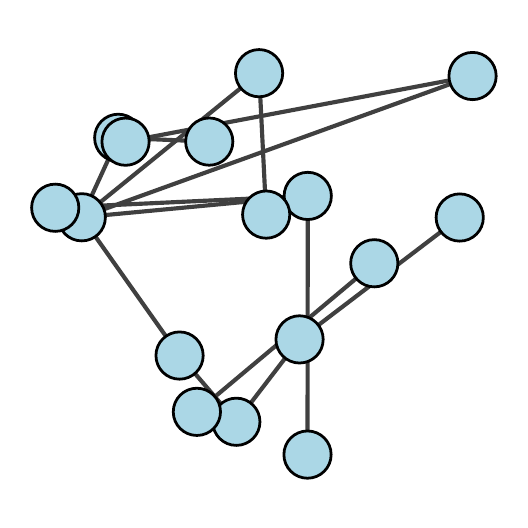
\begin{tikzpicture}
\clip (0,0) rectangle (6,6);
\Vertex[x=1.929,y=1.836]{1}
\Vertex[x=0.687,y=3.592]{7}
\Vertex[x=2.650,y=0.995]{2}
\Vertex[x=3.557,y=3.863]{8}
\Vertex[x=1.150,y=4.601]{11}
\Vertex[x=5.650,y=5.386]{15}
\Vertex[x=1.243,y=4.552]{16}
\Vertex[x=3.453,y=2.041]{3}
\Vertex[x=5.487,y=3.589]{4}
\Vertex[x=2.149,y=1.121]{5}
\Vertex[x=4.402,y=3.008]{6}
\Vertex[x=2.939,y=5.422]{13}
\Vertex[x=3.029,y=3.626]{14}
\Vertex[x=2.306,y=4.553]{12}
\Vertex[x=3.554,y=0.578]{10}
\Vertex[x=0.350,y=3.713]{9}
\Edge[](1)(7)
\Edge[](1)(2)
\Edge[](7)(8)
\Edge[](7)(11)
\Edge[](7)(15)
\Edge[](7)(13)
\Edge[](2)(5)
\Edge[](2)(3)
\Edge[](8)(10)
\Edge[](8)(9)
\Edge[](11)(12)
\Edge[](15)(16)
\Edge[](3)(4)
\Edge[](5)(6)
\Edge[](13)(14)
\end{tikzpicture}
\end{document}